\section{Evaluation}
All calculations and plots are done by Python 3.6.1.
\subsection{Inverting Linear Amplifier}
Note that the used amplifier inverts the signal, transforming a positive input to a negative output and vice versa, but for this evaluation only the absolute
amplification and voltages are used. \\
\noindent
For the first part the frequency response of the input voltage $U_1$ for a resistance ratio of 10 and 100 were measured.
The grade of amplification is adjusted by choosing a corresponding ratio of $\frac{\text{R}_\text{N}}{\text{R}_\text{1}}$ with
${\text{R}_\text{N}}$ = \SI{100}{\kilo\ohm} and ${\text{R}_\text{1}}$ = \SI{10}{\kilo\ohm} for a theoretical amplification of -10, and
${\text{R}_\text{N}}$ = \SI{20}{\kilo\ohm} and ${\text{R}_\text{1}}$ = \SI{0.2}{\kilo\ohm} for -100. These are theoretical because due
to equation (\ref{eq:3}) the neutral amplification $V$ can have an impact on $V'$ and can be approximated with it. For this $V'$ is taken from the measurement at low frequencies. In tabular (\ref{tab:1}) and tabular (\ref{tab:2})
are the measured data of frequency $\nu$, input voltage $U_1$ and output voltage $U_A$.

\begin{minipage}[t]{0.48\linewidth}
\begin{table}[H]
  \centering
  \caption{Data for $\frac{\text{R}_\text{N}}{\text{R}_\text{1}}$ = 10} \label{tab:1}
  \pgfplotstabletypeset[
  col sep=semicolon,
  every head row/.style={
    before row={\toprule
    },
    after row=\hline
  },
  every last row/.style={after row=\bottomrule},
  columns/0/.style={column name=$\nu$ / kHz, column type=c, fixed zerofill, precision=2},
  columns/1/.style={column name= $U_1$ / mV, column type=c, precision=3},
  columns/2/.style={column name=$U_A$ / V, column type=c, fixed zerofill, precision=2},
  ]{a1.csv}
\end{table}
\end{minipage}
\begin{minipage}[t]{0.48\linewidth}
\begin{table}[H]
  \centering
  \caption{Data for $\frac{\text{R}_\text{N}}{\text{R}_\text{1}}$ = 100} \label{tab:2}
  \pgfplotstabletypeset[
  col sep=semicolon,
  every head row/.style={
    before row={\toprule
    },
    after row=\hline
  },
  every last row/.style={after row=\bottomrule},
  columns/0/.style={column name=$\nu$ / kHz, column type=c, fixed zerofill, precision=2},
  columns/1/.style={column name= $U_1$ / mV, column type=c, precision=1, fixed zerofill},
  columns/2/.style={column name=$U_A$ / V, column type=c, fixed zerofill, precision=2},
  fixed
  ]{a3.csv}
\end{table}
\end{minipage}
\vskip 0.2in
\noindent
Looking at the values for the low frequencies, it can be seen that $V'_{10} = 10$  and $V'_{100} = \frac{2}{0.023}$.
Therefore $V'_{10} = \frac{\text{R}_\text{N}}{\text{R}_\text{1}} = \frac{\SI{100}{\kilo\ohm}}{\SI{10}{\kilo\ohm}}$ satisfies for low frequencies, but $V'_{100} = \frac{\text{R}_\text{N}}{\text{R}_\text{1}} = \frac{\SI{20}{\kilo\ohm}}{\SI{0.2}{\kilo\ohm}}$ does not.
Now with equation (\ref{eq:3}) $V$ can be estimated using $V'_{100} = \frac{2}{0.023}$ and $\frac{\text{R}_\text{N}}{\text{R}_\text{1}} = 100$ to
\begin{equation*}
  V = 666,67 \ .
\end{equation*}
\\ \noindent
In figure (\ref{fig:1}) and figure (\ref{fig:2}) is a graphical representation of the data.
\begin{figure}
  \centering
  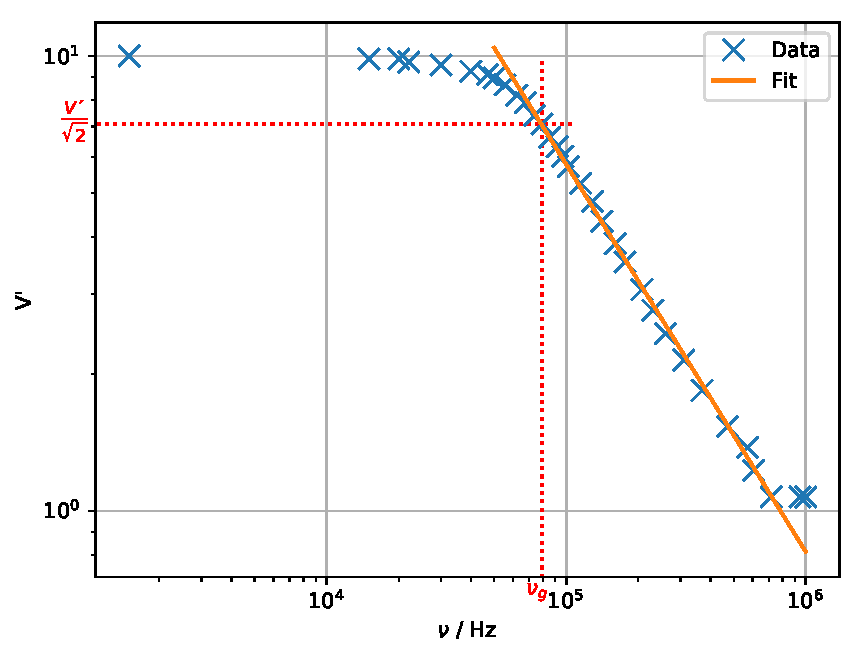
\includegraphics[scale=0.75]{plot1.pdf}
  \caption{Graphical representation of frequency response for $\frac{\text{R}_\text{N}}{\text{R}_\text{1}}$ = 10 ($V'_{10}$)} \label{fig:1}
\end{figure}
The fit curve is a fit of the function
\begin{equation*}
  f(x) = a\cdot x^b
\end{equation*}
and the parameters for $V'_{10}$ are
\begin{align*}
a &= (1.05\pm 0.11)\cdot 10^5 \\
b &= -0.852\pm 0.009 \ .
\end{align*}
In addition the value for $\frac{V'_{10}}{\sqrt{2}} = \frac{10}{\sqrt{2}}$ and its corresponding frequency $\nu'_{g10} = (7.9 \pm 1.4)\cdot 10^4 Hz$ are marked
to compare these to the values for $V'_{100}$.
\begin{figure}[H]
  \centering
  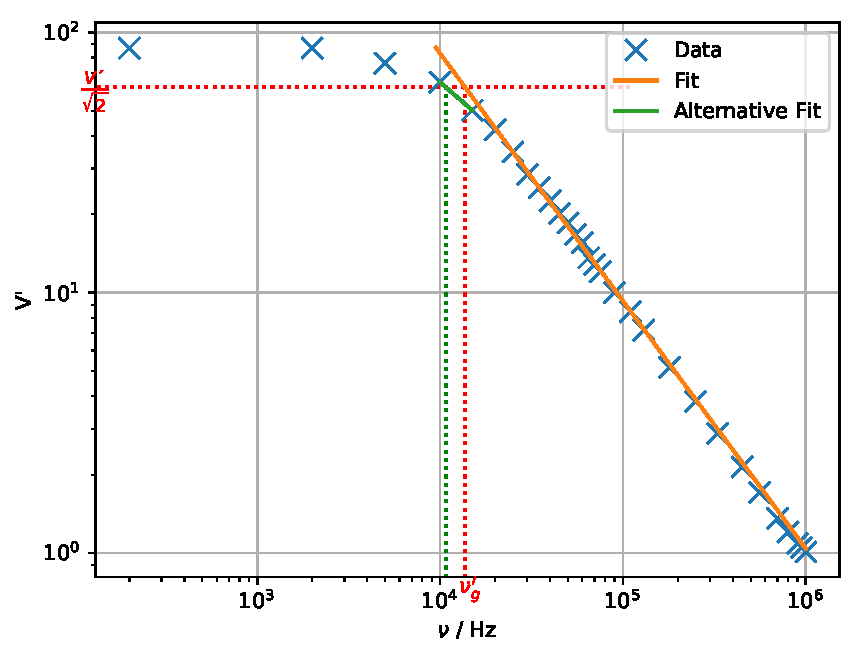
\includegraphics[scale=0.75]{plot3.pdf}
  \caption{Graphical representation of frequency response for $\frac{\text{R}_\text{N}}{\text{R}_\text{1}}$ = 100 ($V'_{100}$)} \label{fig:2}
\end{figure}
\noindent
The parameters for $V'_{100}$ are
\begin{align*}
a &= (5.3\pm 0.5)\cdot 10^5 \\
b &= -0.951\pm 0.009 \ .
\end{align*}
Here the marked value for $\frac{V'_{100}}{\sqrt{2}} = \frac{2}{0.023\cdot \sqrt{2}}$ with its frequency $\nu'_{g100} = (1.37 \pm 0.18)\cdot 10^4 Hz$ can now be
compared to the previous ones to verify the condition of the product of bandwidth and $V'$ being constant.
\begin{align*}
\nu'_{g10} V'_{10} &= (7.9\pm 1.4)\cdot 10^5 Hz \\
\nu'_{g100} V'_{100} &= (1.19+/-0.16)\cdot 10^6 Hz \\
\upDelta &= (51\pm 31) \%
\end{align*}
Looking at figure (\ref{fig:2}) it is clear, that the intersections of $\frac{V'_{100}}{\sqrt{2}}$ with the fitted curve and the direct connection between the data (visualized in green)
are about \SI{3}{\kilo\hertz} apart. This is why an alternative calculation $\nu'_{g100(alt)} V'_{100}$ with $\nu'_{g100(alt)} = \SI{10.8}{\kilo\hertz}$ (approximated through the graph) is done.
\begin{align*}
\nu'_{g10} V'{10} &= (7.9\pm 1.4)\cdot 10^5 Hz \\
\nu'_{g100(alt)} V'{100} &= 9.39\cdot 10^5 Hz \\
\upDelta_{alt} &= (19\pm 21) \%
\end{align*}

\subsection{Terminal Voltage}
The terminal voltage is measured with the inverting linear amplifier, $\nu = \SI{100}{\hertz}$ and a resistance ratio of $\frac{\SI{20}{\kilo\ohm}}{\SI{0.2}{\kilo\ohm}} = 100$ to
% \begin{equation*}
% U_T = \SI{360}{\milli\volt} \.
% \end{equation*}
If a resistance of $\SI{100}{\kilo\ohm}$ is switched in front of the amplifier, then the resistance ratio changes to $\frac{\SI{20}{\kilo\ohm}}{\SI{100.2}{\kilo\ohm}} = 100$ and it follows
\begin{equation*}
U_TR = \SI{15.7}{\milli\volt}
\end{equation*}
For the same procedure for the non-inverting electrometer (same resistance ratio and frequency) the results are
\begin{align*}
U_T &= \SI{3.8}{\volt} \\
U_{TR} &= \SI{3.8}{\volt} \ .
\end{align*}
Note that the absolute values are different due to the amplification done by the oscilloscope to get a visible signal without too much distortion, and only the
relation between the values is important.
The additional resistance has no effect on the electrometer but changes the outcome on the linear amplifier completely. This is because the linear amplifier has
a low input resistance (\approx $\text{R}_\text{1}$) and switching an additional one in series changes the total input resistance a lot. Therefore linear amplifier
is not suitable for measuring high-resistance voltage sources. However the electrometer has a relative high input resistance (\approx \SI{20}{\giga\ohm}) and does not
have these problems and can be used for measuring high-resistance voltage sources.

\subsection{Inverting Integrator}
In tabular (\ref{tab:int}) are the measured data for the inverting integrator.
\begin{table}[H]
  \centering
  \caption{Measurement Data for the inverting integrator} \label{tab:int}
  \pgfplotstabletypeset[
  col sep=semicolon,
  every head row/.style={
    before row={\toprule
    },
    after row=\hline
  },
  every last row/.style={after row=\bottomrule},
  columns/0/.style={column name=$\nu$ / Hz, column type=c },
  columns/1/.style={column name= $U_A$ / V, column type=c, precision=3},
  ]{integrator.csv}
\end{table}
\noindent
In figure (\ref{fig:int}) the data is visualized and the condition of $U_A \sim \frac{1}{\omega}$ can be verified. The operating range
ends approximately where the output voltage reaches a plateau value at about $\nu = \SI{1}{\kilo\ohm}$.
\begin{figure}[H]
\centering
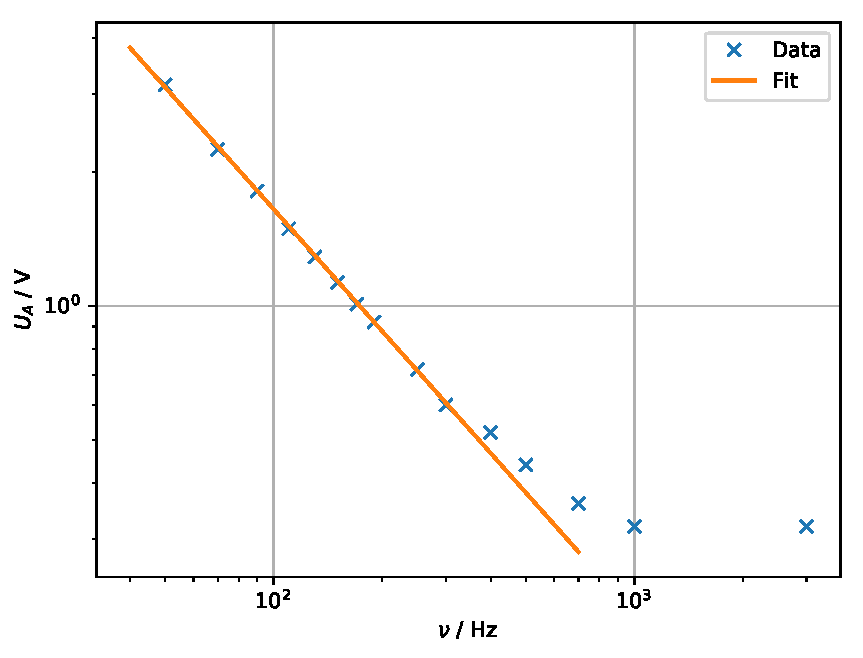
\includegraphics[scale=.75]{plot4.pdf}
\caption{Frequency response of the inverting integrator where $U_A \sim \frac{1}{\omega}$}\label{fig:int}
\end{figure}
\noindent
In figure (\ref{fig:int1}), (\ref{fig:int2}) and (\ref{fig:int3}) is a visualisation of how the inverting integrator works for
a sin voltage, triangular voltage and rectangular voltage.
\begin{figure}[H]
\centering
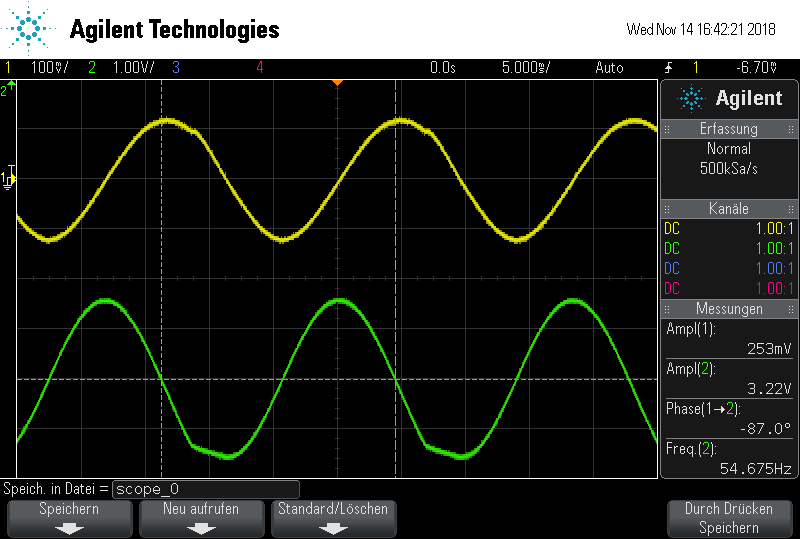
\includegraphics[scale=.48]{V51Bilder/inSin.png}
\caption{Sin voltage integrated}\label{fig:int1}
\end{figure}
\begin{figure}[H]
\centering
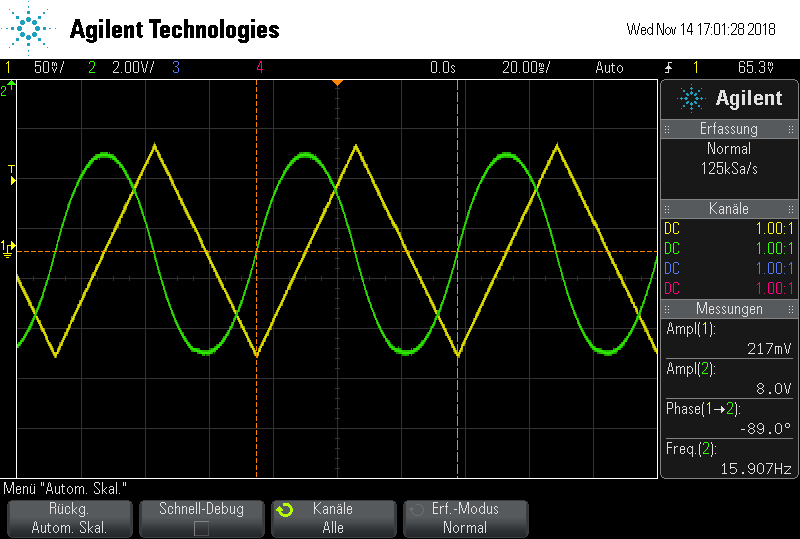
\includegraphics[scale=.48]{V51Bilder/intTri.png}
\caption{Triangular voltage integrated}\label{fig:int2}
\end{figure}
\begin{figure}[H]
\centering
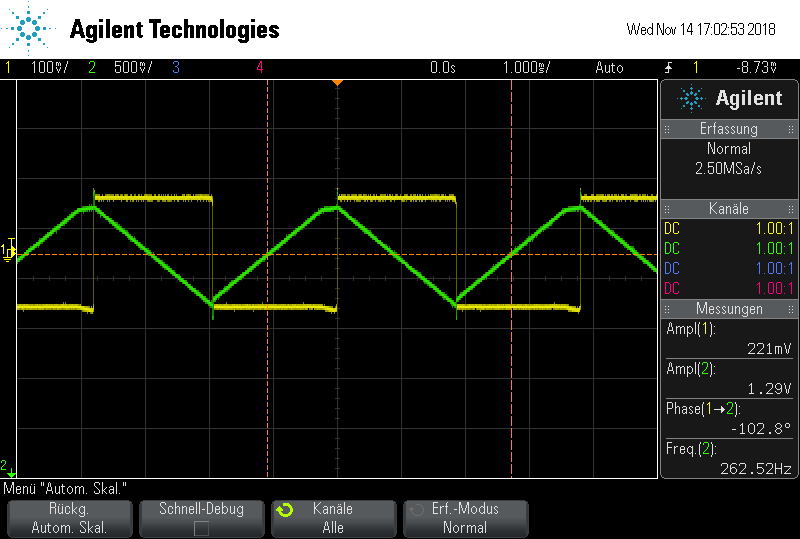
\includegraphics[scale=.48]{V51Bilder/intRect.png}
\caption{Rectangular voltage integrated}\label{fig:int3}
\end{figure}


\subsection{Inverting Differentiator}
In tabular (\ref{tab:diff}) are the measured data for the inverting differentiator.
\begin{table}[H]
  \centering
  \caption{Measurement Data for the inverting differentiator} \label{tab:diff}
  \pgfplotstabletypeset[
  col sep=semicolon,
  every head row/.style={
    before row={\toprule
    },
    after row=\hline
  },
  every last row/.style={after row=\bottomrule},
  columns/0/.style={column name=$\nu$ / Hz, column type=c, },
  columns/1/.style={column name= $U_A$ / mV, column type=c, precision=3},
  ]{differentiator.csv}
\end{table}

\begin{figure}[H]
\centering
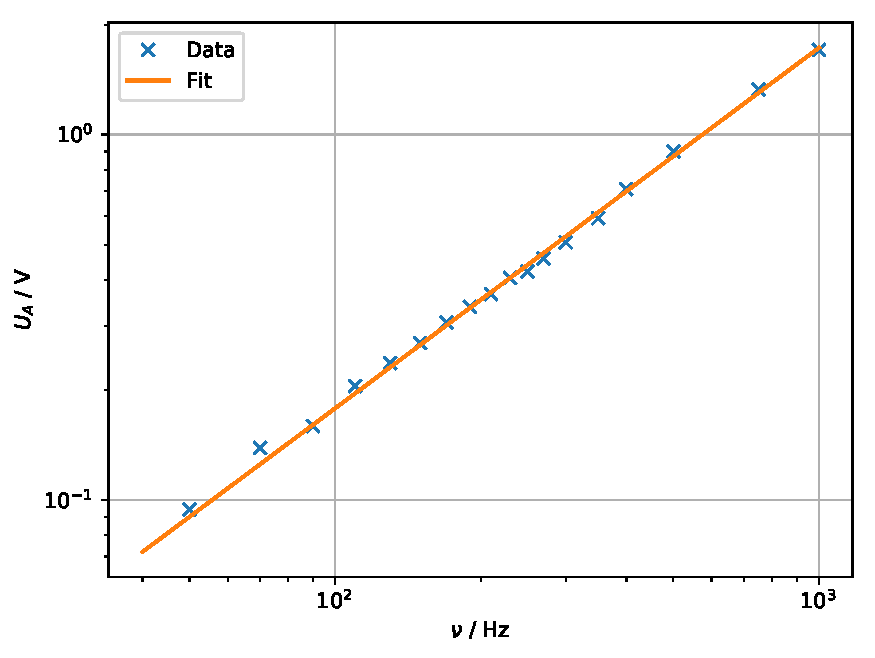
\includegraphics[scale=.75]{plot5.pdf}
\caption{Frequency response of the inverting differentiator where $U_A \sim \omega$}\label{fig:dif}
\end{figure}
\noindent
As no meaningful discrepancy of the fitted curve and the data points is seen, the condition $U_A \sim \omega$ applies for the
whole operating range that has been examined. \\ \noindent
In figure (\ref{fig:diff1}), (\ref{fig:diff2}) and (\ref{fig:diff3}) is a visualisation of how the inverting differentiator works for
a sin voltage, triangular voltage and rectangular voltage.
\begin{figure}[H]
\centering
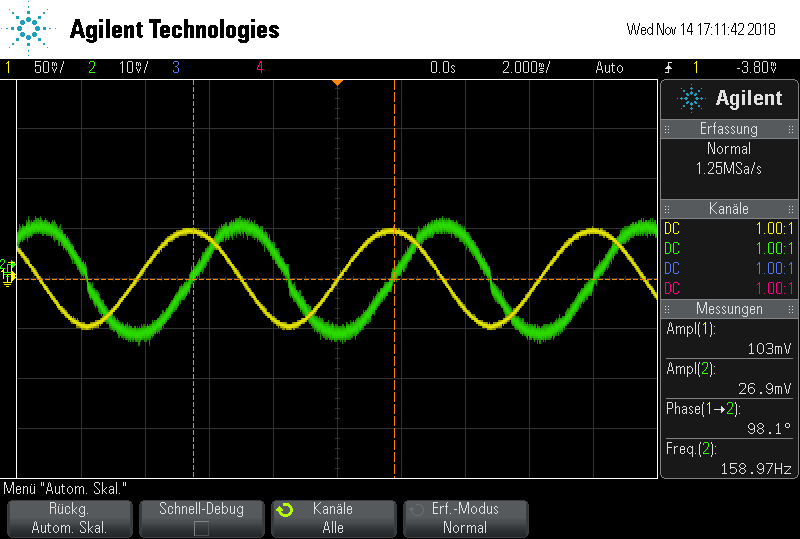
\includegraphics[scale=.48]{V51Bilder/diffSin.png}
\caption{Sin voltage differentiated}\label{fig:diff1}
\end{figure}
\begin{figure}[H]
\centering
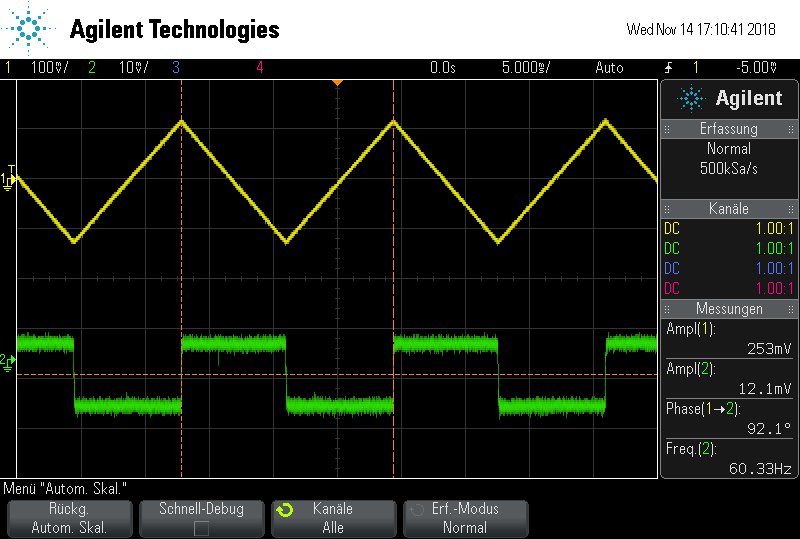
\includegraphics[scale=.48]{V51Bilder/diffTri.png}
\caption{Triangular voltage differentiated}\label{fig:diff2}
\end{figure}
\begin{figure}[H]
\centering
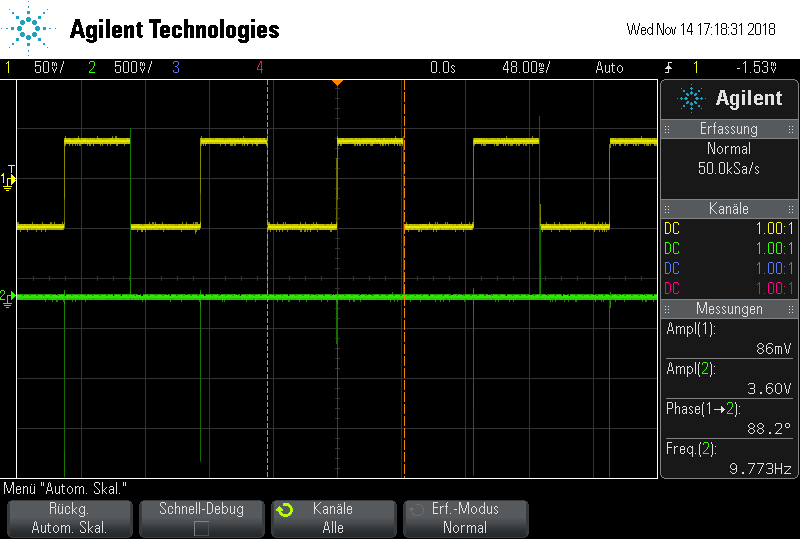
\includegraphics[scale=.48]{V51Bilder/diffRect.png}
\caption{Rectangular voltage differentiated (notice the green spikes)}\label{fig:diff3}
\end{figure}

\subsection{Schmitt-Trigger}
For a resistance ratio of $\frac{\text{R}_\text{1}}{\text{R}_\text{P}} = \frac{\SI{10}{\kilo\ohm}}{\SI{100}{\kilo\ohm}}$ the measurement
for the trigger voltage $U_{B(trigger)}$ and the voltage $2U_B$ gives
\begin{align*}
U_{B(trigger)} &= \SI{1.405}{\volt} \\
2U_B &= \SI{26.9}{\volt} \ .
\end{align*}
The difference between $\frac{\text{R}_\text{1}}{\text{R}_\text{P}}U_B = \SI{1.345}{\volt}$ and $U_{B(trigger)}$ is \SI{4.5}{\percent}.
To see the Schmitt-Trigger in action the trigger effect is visualised in figure (\ref{fig:trig})
\begin{figure}[H]
  \centering
  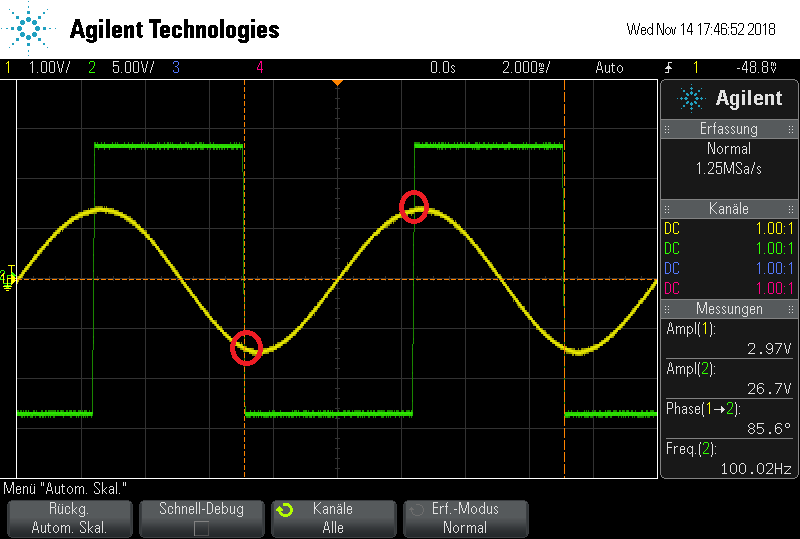
\includegraphics[scale=.9]{V51Bilder/schmitt.png}
  \caption{Visualisation of the trigger effect at a Schmitt-Trigger. (yellow=input, green=output)} \label{fig:trig}
\end{figure}
\noindent
The red circles mark the spots where the input voltage reaches $\pm \frac{\text{R}_\text{1}}{\text{R}_\text{P}}U_B$. Notice
that, once triggered, the output voltage keeps the same as long as the input voltage does not reach the opposing trigger voltage.
Inbetween lies the switch hysterese.
